\documentclass{standalone}
\usepackage[utf8]{inputenc}
\usepackage{pgfplots}
\usetikzlibrary { decorations.pathmorphing, decorations.pathreplacing, decorations.shapes, }

\pgfplotsset{compat=1.3, xlabel=$t$,ylabel=$P$,zlabel=$z$}

\begin{document}
    \pgfplotsset{width=9cm}
    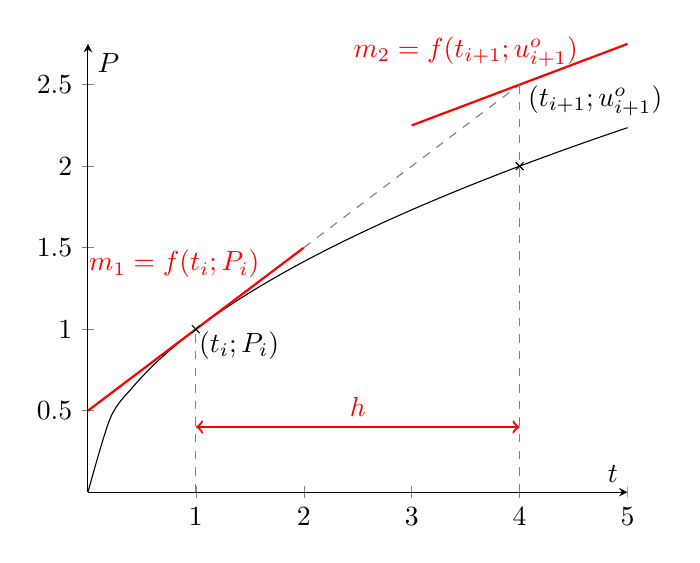
\begin{tikzpicture}
        \begin{axis}[legend cell align=left,
            legend pos=outer north east,ymin=0,xmin=0,
            domain=0:5,clip=false,axis lines=middle]
            \addplot[smooth,color=black] {sqrt(x)};
            \addplot [mark=none,  red,  thick] coordinates { (0,0.5) (2,1.5)}; %m1
            \addplot [mark=none, color=gray, dashed] coordinates { (2,1.5) (4,2.5)};
            \addplot [mark=none,  color=gray,  dashed] coordinates { (1,0) (1,1)}; %punt1
            \addplot [mark=none,  red,  thick] coordinates { (3,2.25) (5,2.75)}; %m2
            \addplot [mark=none,  color=gray,  dashed] coordinates { (4,0) (4,2.5)}; %punt2
            \node at (axis cs:0.8,1.4) [red] {$m_1=f(t_i; P_i)$};
            \node at (axis cs:3.5,2.7) [red] {$m_2=f(t_{i+1}; u^o_{i+1})$};
            \addplot [mark=x] coordinates{(1,1)}; %ti cross
            \node at (axis cs:1.4,0.9) {$(t_i; P_i)$}; %ti name
        %    \addplot [mark=x] coordinates{(4,2.5)}; %ti+1 cross
            \node at (axis cs:4.7,2.4) {$(t_{i+1}; u^o_{i+1})$}; %ti+1 name

            \addplot [mark=x] coordinates{(4,2)}; %P(ti+1) cross
        %    \node at (axis cs:4.8,1.9) {$(t_{i+1}; P(t_{i+1}))$}; %P(ti+1) name
            \addplot [<->, red, thick] coordinates{ (1,0.4) (4,0.4) } node[midway, above]{$h$};
        \end{axis}
    \end{tikzpicture}
\end{document}